%!TEX root = ../dissertation.tex

\chapter{Evaluation}
\label{chapter:evaluation}
% Introduce evaluation...
% Main goals
% Setup used

After the implementation of this solution, explained in chapter \ref{chapter:implementation}, some experiments were performed in order to test it.
The Restaurant and Smart Museum apps, described in section \ref{sec:solution_examples} were used in these experiments. In both, the app tries to scan for the nearest beacon, which means, somehow, it has into account the distance from the beacons.
The library used to handle the beacons has a method to get the distance from a given beacon.
There is a need to check if it is trustworthy the distance's value we get from this library.

The app for end users, described in section \ref{sec:solution_mobile_app_for_end_users}, needs to run, in background, in order to let the user be notified when he/she is nearby any Smart Place, instead of requiring his/her interaction.
However, as any service running in background, it can have a negative impact on the mobile device's resources usage, such as, battery.
A set of experiments was performed to evaluate the overhead introduced by our solution and if it is acceptable, having an app, running in background, scanning for beacons.

A \tm{Motorola}
Moto G\footnote{http://www.gsmarena.com/motorola\_moto\_g-5831.php} smartphone was used to run the mobile application. This device has the following specifications:
\begin{description}
  \item[\gls{CPU}:] Quad-core 1.2 GHz Cortex-A7\footnote{http://www.arm.com/products/processors/cortex-a/cortex-a7.php}
  \item[\gls{GPU}:] Adreno 305
  \item[\gls{RAM}:] 1 \gls{GB}
  \item[Internal storage:]: 16 \gls{GB}
  \item[Screen:] 4.5 inches
  \item[Battery:] Non-removable Li-Ion 2070 \gls{mAh} battery
  \item[\gls{OS}:] Android 5.0.2 (Lollipop\footnote{https://www.android.com/versions/lollipop-5-0})
\end{description}

\section{Methodology}
\label{sec:methodology}
% Previous two problems raised
% Two kinds of experiments
% Tables outlining the experiments
Previously, two problems were raised. First, our solution relies on a library, which its \gls{API} allows us to get the distance from a given beacon.
Second, having the mobile app for end users scanning for beacons periodically can imply some overhead in terms of mobile device's resources usage, such as, battery.
Two experiments were made in order to evaluate the impact of these two problems.

\subsection{Nearest beacon}
\label{sub:methodology_nearest_beacon}
The first set of experiments, summarized in Table~\ref{tab:experiments_nearest_beacon}, try to test if the mobile app can detect the nearest beacon.

\begin{table}[]
\centering
\begin{tabular}{@{}|l|c|c|c|c|@{}}
\toprule
\multicolumn{1}{|c|}{}                & \multicolumn{4}{c|}{{\bf Experiments}}                                                                            \\ \midrule
\multicolumn{1}{|c|}{{\bf Variables}} & {\bf 1}                     & {\bf 2}                   & {\bf 3}                     & {\bf 4}                   \\ \midrule
Events                                & \multicolumn{4}{c|}{\begin{tabular}[c]{@{}c@{}}For each beacon, \\ how many times \\ it was scanned\end{tabular}} \\ \midrule
Number of beacons                     & \multicolumn{4}{c|}{3}                                                                                            \\ \midrule
Interval between each scan (seconds)  & \multicolumn{4}{c|}{10}                                                                                           \\ \midrule
Experiment duration (minutes)         & \multicolumn{4}{c|}{5}                                                                                            \\ \midrule
Distance between beacons (meters)     & \multicolumn{1}{r|}{0.5}    & \multicolumn{1}{r|}{1}    & \multicolumn{1}{r|}{1.5}    & \multicolumn{1}{r|}{2}    \\ \bottomrule
\end{tabular}
\caption[Nearest beacon experiments summary]{Experiments to get the accuracy of the method to get the nearest beacon}
\label{tab:experiments_nearest_beacon}
\end{table}


In these experiments, the Smart Musem example was used.
In each experiment, it ran for 5 minutes. Then, in Android Studio log output, it was possible to check how many times each beacon was detected as the nearest one.

The smartphone and the three beacons were disposed in a layout, where each beacon was equally distant from each other and the smartphone was close to one of them, as shown in Figure~\ref{fig:layout_experiments_nearest_beacon}, where value d, is the distance between beacons.
The names below each beacon (ice, blueberry and mint), were provided by \tm{Estimote} in the developer pack.

In this first set of experiments, the value d starts at 50 centimeters and is increased by 50 centimeters in each experiment until the 4th one where d is 2 meters.

\begin{figure}[!ht]
  \centering
    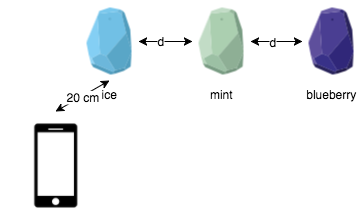
\includegraphics[width=0.5\textwidth, keepaspectratio]{images/nearest_beacon}
    \caption{Layout used for the experiments to get the accuracy of the distance value}
    \label{fig:layout_experiments_nearest_beacon}
\end{figure}

% \subsection{Resources usage}
% \label{sub:methodology_resources_usage}
% The second set of experiments, aims to get a good insight about the overhead introduced by the mobile app that runs on background and scans for beacons periodically. Table~\ref{tab:experiments_resources} summarizes them.
% Here, the three beacons were placed, in the same order as in the experiments described in sub section \ref{sub:methodology_nearest_beacon},
% but the beacons were 25 cm distant from each other. Also, the smartphone was placed in front of the second beacon, as shown in Figure~\ref{fig:experiments_resources_layout}.
%
% \begin{figure}[!ht]
%   \centering
%     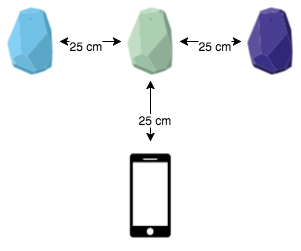
\includegraphics[width=0.5\textwidth, keepaspectratio]{images/experiments_battery_layout}
%     \caption{Layout used for the second and third set of experiments}
%     \label{fig:layout_experiments_resources_layout}
% \end{figure}
%
% In the first half experiments, \gls{WiFi} connection was used and in the remaining ones, \gls{3G} connection was used. These two types of data connection are different, in terms of bandwith, speed, etc. Using these two different connections allowed us to understand if the resources usage is acceptable even if no \gls{WiFi} connection is available. Using Android Studio Device Monitor tool\footnote{http://developer.android.com/tools/help/monitor.html} we were able to collect metrics such as, memory consumption, data network traffic (received and transmitted) and latency of each request.
% Different intervals between each scan were tested to see the impact of its value in the mobile device's resources usage.
% The total experiment duration was ten minutes.
%
% % Please add the following required packages to your document preamble:
% \usepackage{booktabs}
% \usepackage{graphicx}
\begin{table}[]
\centering
\begin{tabular}{@{}|l|c|c|c|c|c|c|@{}}
\toprule
                                     & \multicolumn{6}{c|}{{\bf Experiments}}                                                                                                                      \\ \midrule
{\bf Variables}                      & {\bf 1}                 & {\bf 2}                 & {\bf 3}                  & {\bf 4}                 & {\bf 5}                 & {\bf 6}                  \\ \midrule
Data connection type                 & \multicolumn{3}{c|}{WiFi}                                                    & \multicolumn{3}{c|}{3G}                                                      \\ \midrule
Metrics                              & \multicolumn{6}{c|}{\begin{tabular}[c]{@{}c@{}}CPU usage, memory usage, \\ data network traffic and latency\end{tabular}}                                   \\ \midrule
Number of beacons                    & \multicolumn{6}{c|}{3}                                                                                                                                      \\ \midrule
Interval between each scan (seconds) & \multicolumn{1}{r|}{10} & \multicolumn{1}{r|}{60} & \multicolumn{1}{r|}{300} & \multicolumn{1}{r|}{10} & \multicolumn{1}{r|}{60} & \multicolumn{1}{r|}{300} \\ \midrule
Experiment duration (minutes)        & \multicolumn{6}{c|}{10.5}                                                                                                                                   \\ \midrule
Distance between beacons (meters)    & \multicolumn{6}{c|}{2}                                                                                                                                      \\ \bottomrule
\end{tabular}
\caption{Experiments to evaluate the mobile device's resources usage}
\label{tab:experiments_resources}
\end{table}

%
\subsection{Battery consumption}
\label{sub:methodology_battery_consumption}
One important aspect of this solution is the battery consumption.
Since our mobile app for end users runs on background to scan for nearby beacons, that can have a negative impact on the device's battery. If the user notice that the battery drains too fast, he/she will not use this solution.
Table~\ref{tab:experiments_battery} outlines the experiments performed to evaluate the battery consumption.

% Please add the following required packages to your document preamble:
% \usepackage{booktabs}
\begin{table}[]
\centering
\begin{tabular}{@{}|c|c|c|c|c|@{}}
\toprule
\multicolumn{1}{|l|}{}                     & \multicolumn{4}{c|}{{\bf Experiments}}                                                                \\ \midrule
{\bf Variables}                            & {\bf 1}                  & {\bf 2}                & {\bf 3}                  & {\bf 4}                \\ \midrule
{\bf Data connection type}                 & \multicolumn{2}{c|}{WiFi}                         & \multicolumn{2}{c|}{3G}                           \\ \midrule
{\bf Interval between each scan (minutes)} & \multicolumn{1}{r|}{2.5} & \multicolumn{1}{r|}{5} & \multicolumn{1}{r|}{2.5} & \multicolumn{1}{r|}{5} \\ \midrule
{\bf Experiment duration (hours)}          & \multicolumn{4}{c|}{1}                                                                                \\ \bottomrule
\end{tabular}
\caption[Battery consumption results]{Summary of experiments to get the battery consumption when the mobile
app is scanning for beacons in the background}
\label{tab:experiments_battery}
\end{table}


Figure~\ref{fig:layout_experiments_battery_consumption} shows the layout used for this group of experiments.
There are the same three beacons, as in the the experiments described in section \ref{sub:methodology_nearest_beacon}. The beacons are equally distant, 25 cm, from each other.
The smartphone is at the same distance from the beacon in the middle, the green one named mint.
We performed six experiments. The first two used \gls{WiFi} data connection. The remaining used \gls{3G}.
Using different data connection types allows us to understand if the battery consumption, when the user is not nearby a \gls{WiFi} \gls{AP}.
We tested two values for the interval between each scan, 5 minutes, because it is the default value that the beacons library use in background mode, and 2 and half minutes.
The second value is half the first and we used it to test the impact of this value on battery consumption.

\begin{figure}[!ht]
  \centering
    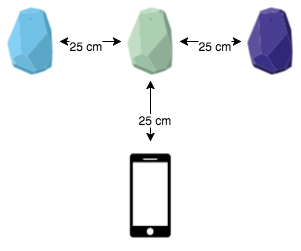
\includegraphics[width=0.5\textwidth, keepaspectratio]{images/experiments_battery_layout}
    \caption{Layout used for the experiments to get the battery consumption}
    \label{fig:layout_experiments_battery_consumption}
\end{figure}

The following scenarios were tested:
\begin{itemize}
  \item When the user stays in the same Smart Place the entire experiment, which lasts one hour;
  \item When the user moves from one Smart Place to another, at each two and half minutes.
\end{itemize}

As already mentioned, for the evaluation process, we have used three \tm{Estimote} beacons.
The mobile app for end users has a cache that stores the beacons that were already scanned.
This way, repeated communications with the backend are avoided.
Data communications, \gls{WiFi} or \gls{3G}, are the major source of battery drain, as suggested in studies, such as \cite{energy}.
To test both scenarios, we would need more than three beacons spread along a big space.
Instead, we simulate the user walking, passing by multiple Smart Places, just by cleaning the cache,
at each two and half minutes.
Doing this, we can guarantee that in most scans, the mobile app will request data from the backend.

In order to get this data, Battery Historian\footnote{https://developer.android.com/tools/performance/batterystats-battery-historian/index.html} was used. This tool allows developers to get the percentage of power drain of any application.

\section{Results}
\label{sec:results}
Previously, in section \ref{sec:methodology} we described the experiments that were used to evaluate the system.
After performed the mentioned experiments, we have got data and taken some conclusions.

\subsection{Nearest Beacon}
\label{sub:results_nearest_beacon}
The mobile app for end users scans for beacons but only requests data for the nearest one. To get the nearest one, it has to rely on the signal strength to calculate the distance. We performed 4 experiments in order to try to get the accuracy of the mechanism that calculates the distance that the mobile device is from a given beacon.
The results of these experiments are summarized in Table~\ref{tab:results_nearest_beacon}, where it is possible to see, for each beacon, how many times it was detected as the nearest one.

Taking into account the layout that was used (see Figure~\ref{fig:layout_experiments_nearest_beacon}), the nearest beacon was the one with name ``ice'' (the blue one).
From Table~\ref{tab:results_nearest_beacon}, it was possible to create the graphic shown in Figure~\ref{fig:results_experiments_nearest_beacon}, which shows that, as we increase the distance between beacons, the accuracy to detect the nearest beacon also increases.

% Please add the following required packages to your document preamble:
% \usepackage{booktabs}
\begin{table}[]
\centering
\begin{tabular}{@{}|c|r|r|r|r|r|@{}}
\toprule
{\bf } & \multicolumn{3}{c|}{{\bf Beacons}} & \multicolumn{2}{c|}{{\bf }} \\ \midrule
{\bf Experiments} & \multicolumn{1}{c|}{{\bf Ice}} & \multicolumn{1}{c|}{{\bf Mint}} & \multicolumn{1}{c|}{{\bf Blueberry}} & \multicolumn{1}{c|}{{\bf Total Scans}} & \multicolumn{1}{c|}{{\bf \% Correct}} \\ \midrule
{\bf 1} & 11 & 7 & 4 & 22 & 50.00\% \\ \midrule
{\bf 2} & 11 & 8 & 0 & 19 & 57.89\% \\ \midrule
{\bf 3} & 14 & 7 & 0 & 21 & 66.67\% \\ \midrule
{\bf 4} & 15 & 1 & 0 & 16 & 93.75\% \\ \bottomrule
\end{tabular}
\caption{Results of experiments about the accuracy to get the nearest beacon}
\label{tab:results_nearest_beacon}
\end{table}


\begin{figure}[!ht]
  \centering
    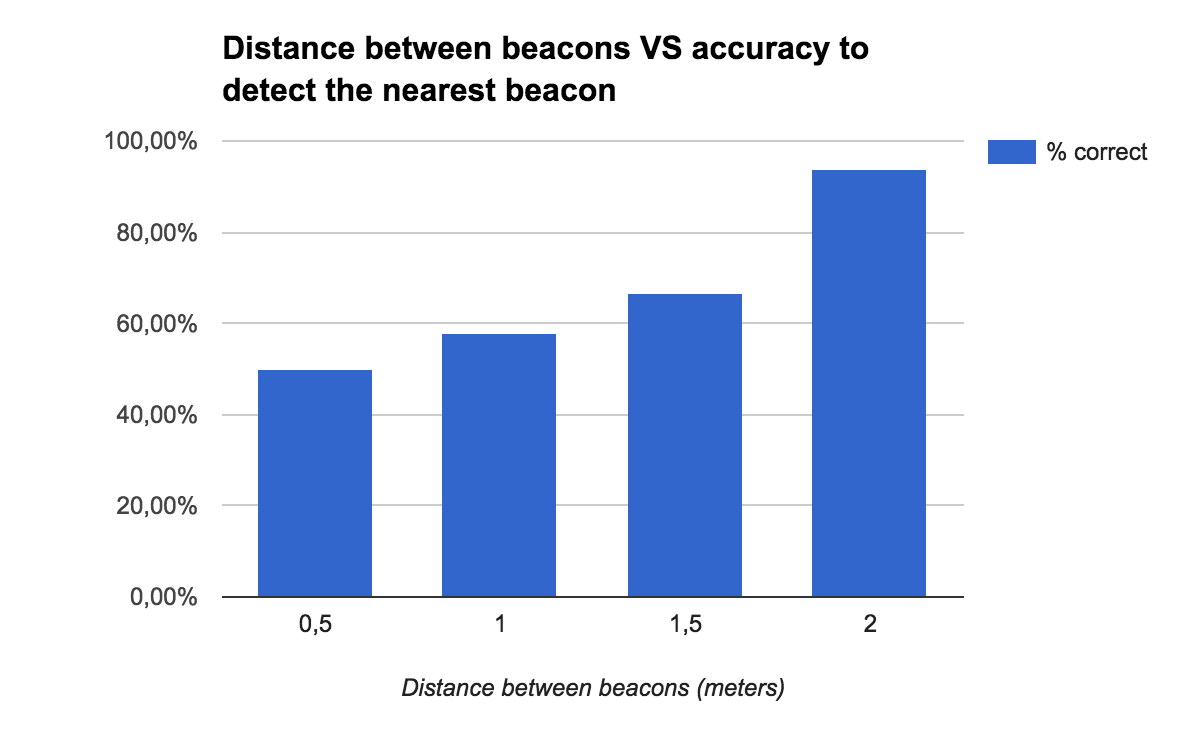
\includegraphics[width=0.5\textwidth, keepaspectratio]{images/results_nearest_beacon}
    \caption{Relation between distance between beacons and accuracy to detect the nearest beacon}
    \label{fig:results_experiments_nearest_beacon}
\end{figure}

In all experiments, this beacon was detected, as the nearest one, at least 50\% off all scans performed.
The only difference between all experiments is the distance between beacons.
We can conclude that, it is recommended that the beacons are, at least, 1.5m or 2m distant from each other.

% \subsection{Resources usage}
% \label{sub:resultsresources_usage}
% We cannot conclude anything here...

\subsection{Battery consumption}
\label{sub:results_battery_consumption}
% As already mentioned... Battery consumption
% Introduce experiments
% Remember the two scenarios
% Results of each scenario
% 3G drains more power
% Results of power drain vs data
As already mentioned, in our solution, there is a mobile app that periodically, scans for beacons, in backgrounds.
As any service running in background, it can imply some overhead in terms of energy.
Following the methodology, explained in section \ref{sub:methodology_battery_consumption}, we evaluated the battery consumption.
For the first scenario, when the user stays in the same Smart Place, during each experiment, the results are summarized in Table~\ref{tab:results_battery_stopped}, where we can see, for each variation of data connection type (\gls{WiFi} and \gls{3G}) and interval between each scan, the values obtained for power drain and data transferred.
From this table, it was possible to create the graphic, shown in Figure~\ref{fig:results_battery_stopped}.
The battery consumption using \gls{WiFi} are almost zero.
However, when using \gls{3G}, the battery consumption raises more than 30 times than using \gls{WiFi}.

% Please add the following required packages to your document preamble:
% \usepackage{booktabs}
\begin{table}[]
\centering
\begin{tabular}{@{}lrrlrr@{}}
\toprule
\textbf{Variables}                                                                          & \multicolumn{5}{c}{\textbf{Results}}                  \\ \midrule
\textbf{Data connection type}                                                               & \multicolumn{2}{c}{WiFi} &   & \multicolumn{2}{c}{3G} \\ \cmidrule{2-3} \cmidrule{5-6}
\textbf{Interval between each scan}                                                         & 2m30s       & 5m         &   & 2m30s      & 5m        \\
\textbf{Computed power drain (\%)}                                                          & 0.00        & 0.00       &   & 0.40       & 0.29      \\
\textbf{\begin{tabular}[c]{@{}l@{}}Data transferred \\ (KB sent and received)\end{tabular}} & 34.96       & 31.10      &   & 21.67      & 35.28     \\ \bottomrule
\end{tabular}
\caption[Power drain when the user is not moving]{Results of the experiments to get the battery consumption in the scenario where the user stays in the same Smart Place}
\label{tab:results_battery_stopped}
\end{table}


\begin{figure}[!ht]
  \centering
    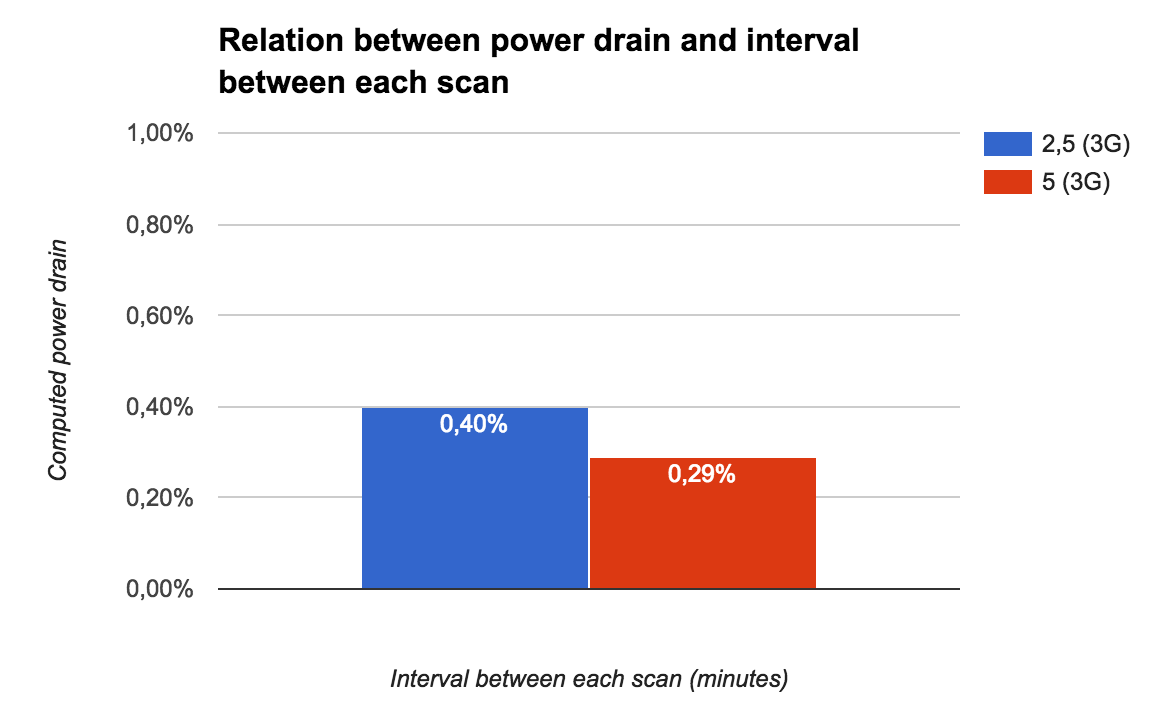
\includegraphics[width=0.8\textwidth, keepaspectratio]{images/results_battery_stopped}
    \caption{Relation between power drain and interval between each scan in the scenario where the user stays in the same Smart Place}
    \label{fig:results_battery_stopped}
\end{figure}

From this results, it is possible to conclude that, our solution, introduces the most overhead when using \gls{3G} as the mean to perform data communications, such as, communications with the backend.
For each data connection type (\gls{WiFi} and \gls{3G}), we tested two values for the interval between each scan for nearby beacons.
We can observe, when we decrease the interval between each scan in half, the battery consumption increases in 0.1\%.
Taking into account that we spent one hour, in each experiment, assuming that the values, for the power drain, grow lineary, it is possible to say that, for two and half and five minutes, in interval between each scan, we would have 6.96\% and 9.6\%, in 24 hours, of power drain, respectively.
The values are still low but, these values can demotivate the usage of our solution, because, it is very likely that the users already have mobile apps, that use mobile data, already installed in their devices, as suggested by Table~\ref{tab:app_comparison}, in chapter \ref{chapter:introduction}, which shows the most popular apps in Google Play Store.

Regarding the second scenario, where the user moves from one Smart Place to another, at each two and half minutes.
Table~\ref{tab:results_battery_walking}, shows the results for this scenario. Here, we got more power drain than in the previous scenario.
These results shows that, the more communication with the backend is required, more power our solution drains.
Once more, using \gls{WiFi}, we have got almost zero power drain.
However, simillary to the results in the previous scenario, there is more power drain using \gls{3G}.
Graphic shown in Figure~\ref{fig:results_battery_walking} shows that, using two minutes and half of interval between each scan, we got more 0.71\% than using five minutes.
As happened before, there is more power drain when we increase the interval between each scan.
Assuming a linear growth of power drain, in the worst case, after 24 hours, there is 65.04\% of power drain.
In this case, we got more than 60 times the power drain than the worst case in the previous scenario.
With this value, our solution can be considered unacceptable for a daily basis usage, that is, having the mobile app always running in background.

% Please add the following required packages to your document preamble:
% \usepackage{booktabs}
\begin{table}[]
\centering
\begin{tabular}{@{}|l|r|r|r|r|@{}}
\toprule
{\bf }                                        & \multicolumn{4}{c|}{{\bf Results}}                  \\ \midrule
{\bf Data connection type}                    & \multicolumn{2}{c|}{WiFi} & \multicolumn{2}{c|}{3G} \\ \midrule
{\bf Interval between each scan (minutes)}    & 2.5         & 5           & 2.5         & 5         \\ \midrule
{\bf Computed power drain (\%)}               & 0.01        & 0.01        & 2.71        & 2.00      \\ \midrule
{\bf Data transferred (KB sent and received)} & 71.44       & 67.86       & 229.96      & 138.26    \\ \bottomrule
\end{tabular}
\caption[Power drain when the user is moving]{Results of the experiments to get the battery consumption in the scenario where the user is moving along multiple Smart Places}
\label{tab:results_battery_walking}
\end{table}


\begin{figure}[!ht]
  \centering
    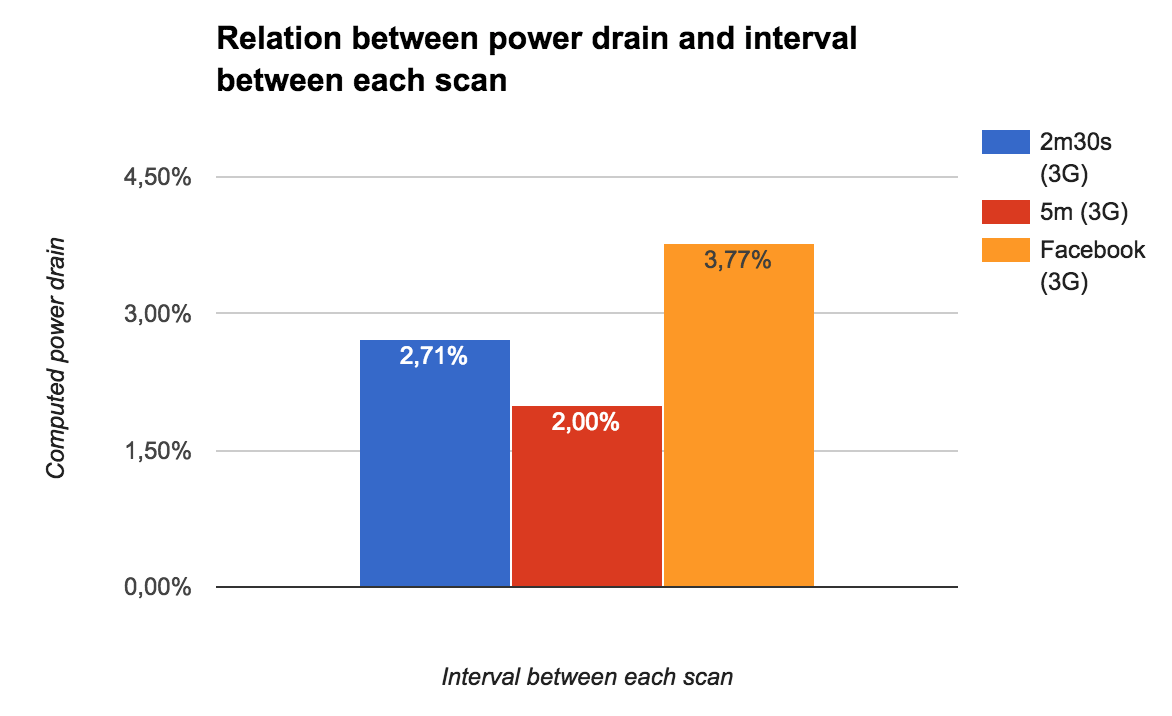
\includegraphics[width=0.8\textwidth, keepaspectratio]{images/results_battery_walking}
    \caption{Relation between power drain and interval between each scan in the scenario where the user moves along multiple Smart Places}
    \label{fig:results_battery_walking}
\end{figure}

Looking at the results, it is possible to establish a relation between power drain and data transferred (sent and received).
In all experiments, we got how many \gls{KB} were transferred.
Since, when using \gls{WiFi}, the power drain was almost zero, we have focused in the relation between power drain and data transferred using \gls{3G}.
As the graphic, in Figure~\ref{fig:results_battery_data}, shows, as more data is transferred, more power, of the mobile device, is drained.
It is possible to conclude that, the more our mobile app needs to communicate with the backend, the more is the energy consumption.

\begin{figure}[!ht]
  \centering
    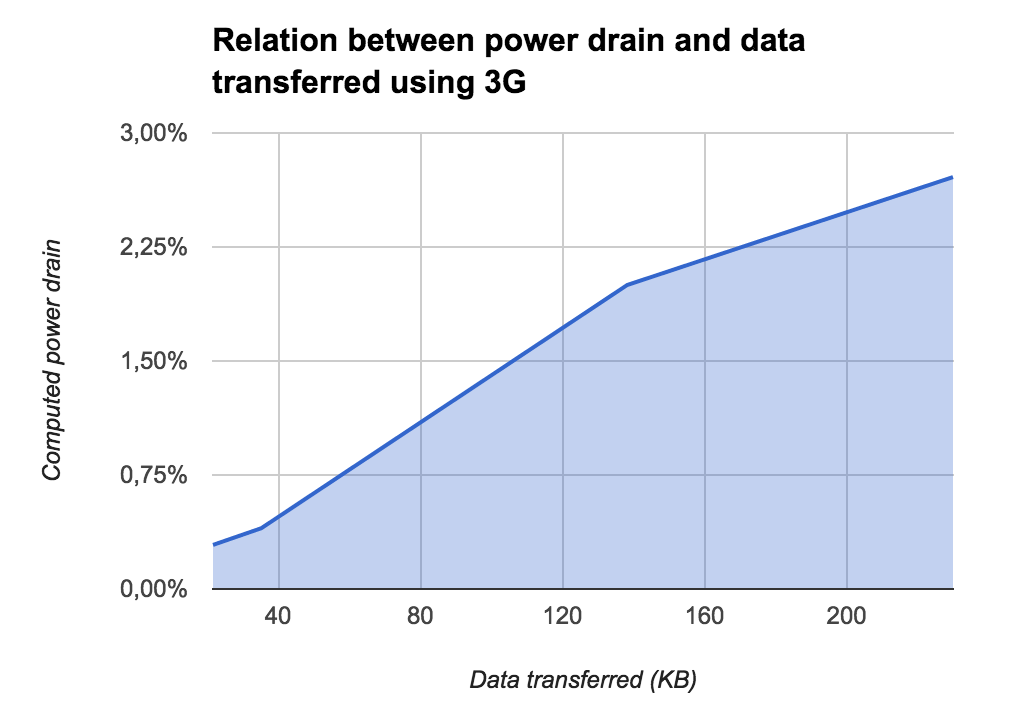
\includegraphics[width=0.8\textwidth, keepaspectratio]{images/results_battery_data}
    \caption{Relation between power drain and data transferred}
    \label{fig:results_battery_data}
\end{figure}

% \section{Conclusions}
% \label{sec:conclusions}
% % Outline experiments for nearest beacon
% % Take care of distance
% % Outline experiments for battery consumption
% % In some cases, having the app always turned on, can be unnaceptable
% In the solution we have been developing, there were two problems
